\documentclass[aspectratio=169,12pt]{beamer}
\usepackage[utf8]{inputenc}
\usepackage[spanish, es-nodecimaldot]{babel}
%\usepackage{icomma} % Use dot as decimal separator
\usepackage{booktabs} % For better-looking tables
\usepackage{wrapfig}
\usepackage{caption}
%\usepackage{siunitx}


\usepackage{refcount}

\usepackage{multicol}
\usepackage{mathtools}

\usepackage[normalem]{ulem}

\pagestyle{empty}

\usepackage{pgf,tikz}
\usepackage{pgfplots}
\usetikzlibrary{matrix}
\usetikzlibrary{arrows}

%\usepackage{wrapfig}
\mode<presentation>
\usefonttheme{professionalfonts}
\usetheme{Darmstadt}
\usecolortheme{orchid}
\useoutertheme{default}
\setbeamertemplate{headline}{}

\renewcommand{\baselinestretch}{1.1}

%gets rid of bottom navigation bars
\setbeamertemplate{footline}[page number]

%gets rid of navigation symbols
\setbeamertemplate{navigation symbols}{}

%\frameframe{none} % No default frame

%\setlength{\framewidth}{8.7in} \setlength{\frameheight}{7.2in}

\parindent 0pt
\setlength{\parskip} {1ex plus 0.5ex minus 0.2ex}


%\usepackage[bbgreekl]{mathbbol}
\usepackage{amsfonts}

%\DeclareSymbolFontAlphabet{\mathbb}{AMSb}
%\DeclareSymbolFontAlphabet{\mathbbl}{bbold}

\newcommand{\Sym}{{\mathcal S}}
\DeclareMathOperator{\Aut}{Aut}
\DeclareMathOperator{\Tr}{Tr}
\DeclareMathOperator{\trace}{Trace}
\DeclareMathOperator{\range}{range}
\DeclareMathOperator{\rank}{rank}

\usepackage{breqn}
\usepackage{multicol}
\usepackage{colortbl}
\usepackage{lmodern}
\usepackage{tabularx}
\usepackage{multirow}
\usepackage{amssymb}
\usepackage{amsmath}
\usepackage{stmaryrd}
\usepackage{color}
\usepackage{graphicx}
\graphicspath{ {img/} }
\usepackage{hyperref}

\input{epsf}
\title{Introducción}
\author{}

\DeclareMathOperator{\Hom}{Hom}
\DeclareMathOperator{\sing}{sing}

\DeclareMathOperator{\chara}{char}
\DeclareMathOperator{\Jacob}{Jacob}
\DeclareMathOperator{\Sing}{Sing}
\newcommand{\fracNoLine}[2]{\genfrac{}{}{}{0pt}{#1}{#2}}

%\beamerdefaultoverlayspecification{<+->}

\usepackage{listings,xcolor,bm}


\definecolor{mygreen}{rgb}{0,0.6,0}
\definecolor{mygray}{rgb}{0.5,0.5,0.5}
\definecolor{mymauve}{rgb}{0.58,0,0.82}
\lstset{
  backgroundcolor=\color{white},   % choose the background color; you must add
  basicstyle=\small\ttfamily,      % the size of the fonts that are used for the code
  breakatwhitespace=false,         % sets if automatic breaks should only happen at whitespace
  breaklines=true,                 % sets automatic line breaking
  captionpos=b,                    % sets the caption-position to bottom
  commentstyle=\color{mygreen},    % comment style
  deletekeywords={...},            % if you want to delete keywords from the given language
  escapeinside={\%*}{*)},          % if you want to add LaTeX within your code
  extendedchars=true,              % lets you use non-ASCII characters; for 8-bits encodings only, does not work with UTF-8
  firstnumber=1,                % start line enumeration with line 1000
  frame=single,	                   % adds a frame around the code
  keepspaces=true,                 % keeps spaces in text, useful for keeping indentation of code (possibly needs columns=flexible)
  keywordstyle=\color{blue},       % keyword style
  language=Python,                 % the language of the code
  morekeywords={*,...},            % if you want to add more keywords to the set
  numbers=left,                    % where to put the line-numbers; possible values are (none, left, right)
  numbersep=5pt,                   % how far the line-numbers are from the code
  numberstyle=\tiny\color{mygray}, % the style that is used for the line-numbers
  rulecolor=\color{black},         % if not set, the frame-color may be changed on line-breaks within not-black text (e.g. comments (green here))
  showspaces=false,                % show spaces everywhere adding particular underscores; it overrides 'showstringspaces'
  showstringspaces=false,          % underline spaces within strings only
  showtabs=false,                  % show tabs within strings adding particular underscores
  stepnumber=5,                    % the step between two line-numbers. If it's 1, each line will be numbered
  stringstyle=\color{mymauve},     % string literal style
  tabsize=4,	                   % sets default tabsize to 2 spaces
  title=\lstname                   % show the filename of files included with \lstinputlisting; also try caption instead of title
}

\begin{document}

\newtheorem{prop}{Proposici\'on}
\newtheorem{algo}[prop]{Algorithm}
\newtheorem{teor}[prop]{Theorem}
\newtheorem{lema}[prop]{Lemma}
\newtheorem{coro}[prop]{Corollary}
\newtheorem{defi}[prop]{Definition}

\newcommand{\ideal}[1]{{\left\langle{#1}\right\rangle}}
\newcommand{\demo}{\textbf {Demostraci\'on. }}
\newcommand{\obse}{\textbf {Observaci\'on. }}
\newcommand{\Input}{\textbf {Input: }}
\newcommand{\Output}{\textbf {Output: }}
\newcommand{\Examp}{\textbf {Ejemplo }}
\newcommand{\Examps}{\textbf {Ejemplos }}

\newcommand{\kk}{{\mathbbl k}}
\newcommand{\V}{{\mathbf V}}
\newcommand{\I}{{\mathbf I}}
\newcommand{\PP}{{\tilde P}}
\newcommand{\QQ}{{\tilde Q}}

\newcommand{\F}{{\mathbb F}}
\newcommand{\Q}{{\mathbb Q}}
\newcommand{\N}{{\mathbb N}}
\newcommand{\R}{{\mathbb R}}
\newcommand{\Z}{{\mathbb Z}}
\newcommand{\CC}{{\mathbb C}}
\newcommand{\eLL}{{\mathcal L}}



\newcommand{\MinAss}{\textrm {MinAss}}
\newcommand{\Ass}{\textrm {Ass}}
\newcommand{\mcm}{\textrm {mcm}}
\newcommand{\mcd}{\textrm {mcd}}
%\newcommand{\mod}{\textrm { mod }}
\newcommand{\lt}{\textrm {lt}}
\newcommand{\Lt}{\textrm {Lt}}
\newcommand{\lp}{\textrm {lp}}
\newcommand{\lc}{\textrm {lc}}
\newcommand{\lm}{\textrm {lm}}
\newcommand{\barra}{\ /\ }
\newcommand{\multideg}{\textrm {multideg}}

\newcommand{\sep}{\textrm {sep}}
\newcommand{\Syz}{\textrm {Syz}}
\newcommand{\n}{\~n}
\newcommand{\cG}{\textrm {cG}}
\newcommand{\dG}{\textrm {dG}}
\newcommand{\nG}{\textrm {nG}}
\newcommand{\CE}{\textrm {CE}}
\newcommand{\CG}{\textrm {CG}}
\newcommand{\CF}{\textrm {CF}}
\newcommand{\DG}{\textrm {DG}}
\renewcommand{\NG}{\textrm {NG}}

\newcommand{\p}{{\boldsymbol{p}}}
\newcommand{\q}{{\boldsymbol{q}}}

\newcommand{\X}{{\boldsymbol{X}}}
\newcommand{\x}{{\boldsymbol{x}}}
\renewcommand{\u}{{\boldsymbol{u}}}
\renewcommand{\t}{{\boldsymbol{t}}}
\renewcommand{\a}{{\boldsymbol{a}}}
\renewcommand{\b}{{\boldsymbol{b}}}
\renewcommand{\c}{{\boldsymbol{c}}}

%Titulos en espa�ol
%\renewcommand{\chaptername}{Cap\'{\i}tulo}
%\renewcommand{\bibname}{Bibliograf\'{\i}a}

\newcommand{\kring}{\kk[\x]}
\newcommand{\kRing}{\kk[X]}
\newcommand{\qring}{\Q[\x]}

%\renewcommand\itemindent{-10pt}
%\renewcommand{\theenumi}{\arabic{enumi}}
%\renewcommand{\labelenumi}{\Alph{enumi}}

\definecolor{issac}{rgb}{1.00,0.00,0.00}
%------------------------------------------------------------------

\begin{frame}

 \begin{center}

\Large\textbf{Laboratorio de Datos} \\
\large\textbf{Entrenamiento y testeo}
%\vspace{0.5cm}

% \textit{Santiago Laplagne} \\
%slaplagn@dm.uba.ar \\


%\vspace{0.5cm}
%{\small Trabajo en progreso en conjunto con \emph{Jose Capco} (Universit\"at Innsbruck) y \emph{Claus Scheiderer} %(Universit\"at Konstanz).} \\

\vspace{1cm}
Primer Cuatrimestre 2024 \\ Turnos tarde y noche

\vspace{1cm}


 {\small Facultad de Ciencias Exactas y Naturales, UBA}
 \end{center}


\end{frame}

%------------------------------------------------------------------

\begin{frame}
\frametitle{Aprendizaje Supervisado y No Supervisado}
\begin{columns}
    \column{0.5\textwidth}
    \textbf{Aprendizaje Supervisado:}
    \begin{itemize}
        \item El objetivo es predecir una variable respuesta a partir de variables explicativas.
        \item Conocemos la respuesta correcta para un conjunto de datos y usamos esos datos para construir el modelo.
        \item Ejemplos: regresión, clasificación.
    \end{itemize}

    \column{0.5\textwidth}
    \textbf{Aprendizaje No Supervisado:}
    \begin{itemize}
        \item El objetivo es encontrar patrones o estructuras ocultas en los datos.
        \item No conocemos o no hay a priori una respuesta correcta.
        \item Ejemplos: agrupación (clustering), reducción de dimensionalidad.
    \end{itemize}
\end{columns}
\end{frame}


\begin{frame}
\frametitle{Introducción a la Agrupación}

En las últimas clases estudiamos modelos de regresión (aprendizaje supervisado).

Estudiamos ahora métodos de agrupamiento(clustering).

\begin{minipage}{.5\textwidth}
\begin{itemize}
    \item La agrupación es una técnica de aprendizaje no supervisado.
    \item El objetivo es agrupar datos similares en conjuntos llamados clústeres.
    \item Aplicaciones: segmentación de mercado, análisis de redes sociales, imagenes médica, etc.
\end{itemize}
\end{minipage}%
\begin{minipage}{.5\textwidth}
\begin{center}
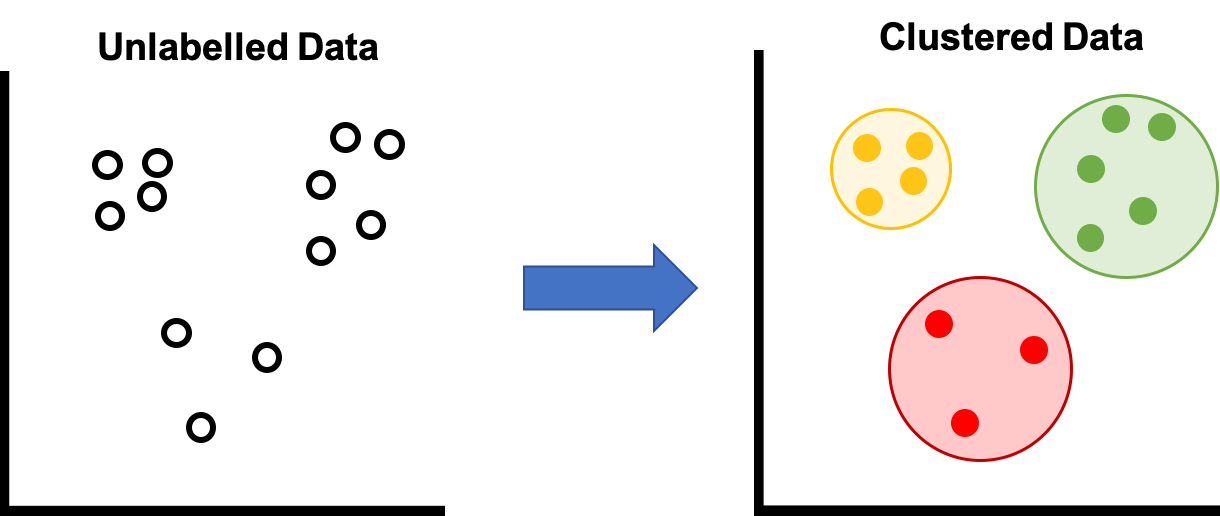
\includegraphics[scale=0.15]{clase15-labelledData.png}
\end{center}
\end{minipage}%


\end{frame}

\begin{frame}
\frametitle{Aplicaciones: segmentación de mercado}

\begin{center}
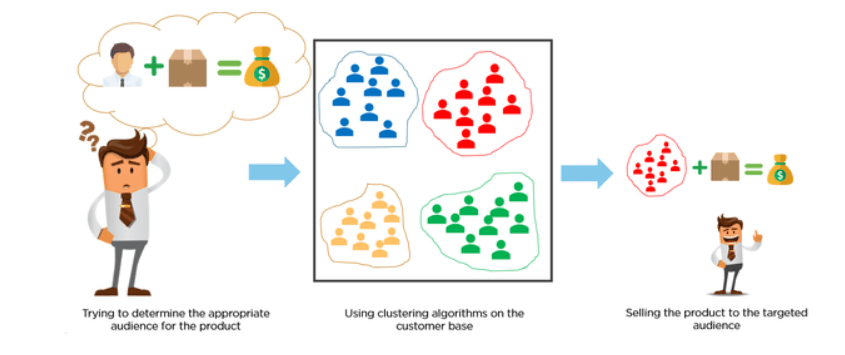
\includegraphics[scale=0.5]{clase15-Customer_Segmentation.png}
\end{center}


\end{frame}

\begin{frame}
\frametitle{Aplicaciones: imágenes médicas}

\begin{center}
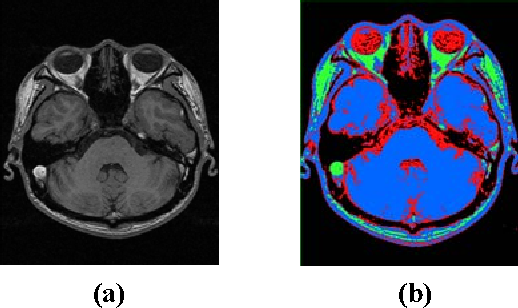
\includegraphics[scale=0.5]{clase15-clustering-imagenesMedicas.png}
\end{center}


\end{frame}


\begin{frame}
\frametitle{Clustering por $K$-medias ($K$-means}

Existen diversos algoritmos de clustering.

\begin{itemize}
    \item K-means es un algoritmo de agrupación que particiona los datos en $k$ clústeres.
    \item Se definen $k$ centros para los clusters.
    \item Para determinar el cluster al que corresponde cada elemento, se busca cuál es el centro más cercano.
\end{itemize}
\end{frame}


\begin{frame}
\frametitle{Procedimiento de K-means}
\begin{enumerate}
    \item Elegir $k$ centroides iniciales aleatoriamente.
    \item Asignar cada punto de datos al clúster más cercano (basado en la distancia euclidiana).
    \item Calcular nuevos centroides como la media de los puntos asignados a cada clúster.
    \item Repetir los pasos 2 y 3 hasta que los centroides no cambien significativamente.
\end{enumerate}
\end{frame}


\begin{frame}
\frametitle{Ventajas y Desventajas de K-means}
\begin{columns}
    \column{0.5\textwidth}
    \textbf{Ventajas:}
    \begin{itemize}
        \item Simple y fácil de implementar.
        \item Escalable para grandes conjuntos de datos.
    \end{itemize}
    \column{0.5\textwidth}
    \textbf{Desventajas:}
    \begin{itemize}
        \item Requiere especificar el número de clústeres ($k$) de antemano.
        \item Sensible a la elección de los centroides iniciales.
        \item Puede converger a mínimos locales.
    \end{itemize}
\end{columns}
\end{frame}


\begin{frame}[fragile]
\frametitle{Aplicación de K-means en Python}
\begin{itemize}
    \item Ejemplo de implementación en Python usando \texttt{scikit-learn}:
\end{itemize}

\begin{lstlisting}
from sklearn.cluster import KMeans
import numpy as np

# Datos de ejemplo
X = np.array([[1, 2], [1, 4], [1, 0],
              [10, 2], [10, 4], [10, 0]])

# Inicializar K-means
kmeans = KMeans(n_clusters=2, random_state=0).fit(X)

# Resultados
print(kmeans.labels_)
print(kmeans.cluster_centers_)
\end{lstlisting}

\end{frame}

\end{document}
